\section{Grundlagen}
Dieses Kapitel besch\"aftigt sich mit den Grundlagen, die f\"ur diese Arbeit relevant sind. Dabei geht es sowohl um die Entwicklungsumgebung Unity3D, als auch um das Konzept der Triangluar Meshes, die essenziell in der 3D-Computergrafik sind.

\subsection{Unity3D}
Unity3D ist eine plattform\"ubergreifende Spiele-Engine mit eingebauter Entwicklungsumgebung f\"ur zwei- und dreidimensionale, sowie Augmented- und Virtual-Reality Spiele und Simulationen. Die Engine besitzt einen eigenen Editor, in dem diverse Szenarien erstellt und bearbeitet werden k\"onnen. Um diese Szenarien zum Leben zu erwecken unterst\"utzt Unity selbst programmierte Scripte auf der Grundlage von C\#. Insgesamt laufen auf \"uber drei Milliarden Ger\"aten Programme, die mit Unity erstellt wurden, auf \"uber 25 verschiedenen Plattformen, wie Windows oder Linux und den g\"angigen Spielekonsolen wie die PlayStation 4, XBox One und der Nintendo Switch. Zudem sind 50\% aller mobilen Spiele und 60\% aller VR/AR Anwendungen mithilfe von Unity entstanden \cite{Unity}. Spiele wie ,,Pok\'emon Go'', ,,Superhot'' und das Simulationsspiel ,,Universe Sandbox'' sind drei Beispiele f\"ur Spiele, die in Unity erstellt wurden.

\subsection{Triangular Meshes}
Um auf einem Computer eine dreidimensionale Szene, zum Beispiel mit der Hilfe von Unity darzustellen, m\"ussen alle dargestellten Modelle angen\"ahert werden. In der Regel werden daf\"ur Dreiecksnetze (Triangular Mesh) verwendet, die die Oberfl\"ache eines Objekts mithilfe von Dreiecken ann\"ahert, wie in Abbildung \ref{fig:dolphintrianglemesh} anhand eines Delfins gezeigt. Informationen, die f\"ur ein solches Dreiecksnetz garantiert ben\"otigt werden, sind eine Reihe von Eckpunkten, den Vertices, die immer in Dreiermengen kommen und deren Position im dreidimensionalen Raum \cite[S.262]{Shirley2010}. Diese werden durch Kanten (Edges) verbunden und bilden damit Dreiecksfl\"achen, auch Faces genannt.

\begin{figure}[h]
	\centering
	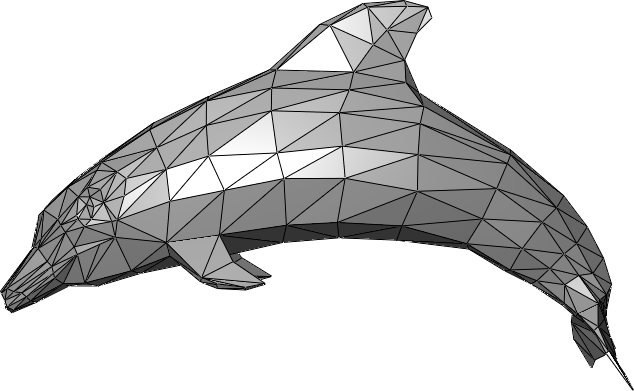
\includegraphics[width=0.7\linewidth]{Images/Dolphin_triangle_mesh}
	\caption[Beispiel eines Polygonen-Netzes]{Beispiel eines Dreiecks-Polygonen-Netz, von \cite{WikipediaDolphin1}}
	\label{fig:dolphintrianglemesh}
\end{figure}


Die einfachste Implementierung eines solchen Meshes sieht vor, f\"ur jedes Dreieck drei Punkte mit jeweils einer X-, Y- und Z-Koordinate zu speichern. Wichtig ist, dass die Orientierung der Dreiecke immer gleich bleibt, also dass im gesamte Netz die Punkte aller Dreiecke im oder gegen den Uhrzeigersinn angegeben sind. Eine konsequente Behandlung der Orientierung der Dreiecke ist f\"ur jede Art von Mesh wichtig. Ein Nachteil von dieser Art, ein Mesh zu speichern ist, dass Punkte die h\"aufig im Netz vorkommen mehrfach gespeichert werden. 

Aus diesem Grund kann eine abgewandelte Version davon verwendet werden, ein Indexed Mesh. Ein solches Mesh trennt die Vertices von der Verwendung im Mesh. Daf\"ur werden zwei Listen verwendet, eine mit den Punkten und eine Liste mit den Indices, wie die Dreiecke zu konstruieren sind. Ein Index zeigt auf eine Position in der Vertex-Liste und drei Indices formen jeweils eine Face \cite[S.265]{Shirley2010}.

\subsection{Triangular Meshes in Unity}
Unity bietet die M\"oglichkeit, mit Hilfe von selbstgeschriebenen Scripten eigene Indexed Meshes zu erstellen. Daf\"ur stellt Unity ein eigenes Mesh-System zur Verf\"ugung, die \textit{UnityEngine.Mesh}-Klasse. Damit diese ein Mesh rendern kann, erwartet das Mesh zum einen ein \textit{UnityEngine.Vector3}-Array f\"ur die Vertices, wobei ein \textit{Vector3} ein Punkt im dreidimensionalen Raum darstellt. Zum anderen erwartet es ein \textit{int}-Array, welches die Reihenfolge der Eckpunkte festlegt, indem die Indizes der zu verwendenden Vertices angegeben werden. Zu beachten ist, dass die Vertices eines Unity-Meshs immer im Uhrzeigersinn orientiert sind, im Gegensatz zu Anwendungen wie Blender, die gegen den Uhrzeigersinn arbeiten.
  
Der folgende Code zeigt beispielhaft, wie ein Unity-Mesh erzeugt werden kann:
\begin{lstlisting}
public void CreateMesh()
{
	//--- Der Vollstaendigkeit halber vorhanden
	meshFilter = gameObject.GetComponent<MeshFilter>();
	if (meshFilter == null)
	meshFilter = gameObject.AddComponent<MeshFilter>();

	//--- vom MeshFilter zum Mesh
	mesh = meshFilter.sharedMesh;
	if (mesh == null)
		mesh = new Mesh { name = "Quad" };

	//--- MeshRenderer holen
	meshRenderer = this.gameObject.GetComponent<MeshRenderer>();
	if (meshRenderer == null)
		meshRenderer = gameObject.AddComponent<MeshRenderer>();

	//--- Mesh zusammenstellen
	//--- Vertices/Points
	Vector3 P0 = new Vector3(0, 0, 0);
	Vector3 P1 = new Vector3(0, 1, 0);
	Vector3 P2 = new Vector3(1, 0, 0);
	Vector3 P3 = new Vector3(1, 1, 0);

	List<Vector3> verticies = new List<Vector3> { P0, P1, P2, P3 };

	//--- Triangles
	List<int> triangles = new List<int> 
		{0, 1, 2, 	// --- Dreieck 1
		 2, 1, 3};	// --- Dreieck 2

	//--- Mesh bef\"ullen
	mesh.Clear();
	//--- Vertices zuweisen
	mesh.vertices = verticies.ToArray();
	//--- Triangles zuweisen
	mesh.triangles = triangles.ToArray();
	//--- Mesh dem MeshFilter zuweisen
	meshFilter.sharedMesh = mesh;
}
\end{lstlisting}

Und liefert folgendes Ergebnis:
\begin{figure}[h]
	\centering
	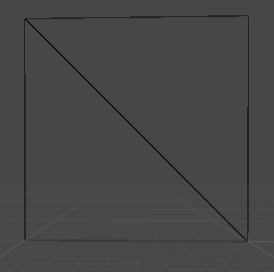
\includegraphics[width=0.35\linewidth]{Images/UnityQuadWireframe}
	\caption[Die Wireframeansicht des erstellten Meshes]{Die Wireframeansicht des erstellten Meshes im Unity Editor}
	\label{fig:unityquadwireframe}
\end{figure}

\subsection{Datenstrukturen f\"ur Meshes}
Wird zur Laufzeit eine Nachbarschaftsbeziehung abgefragt, zum Beispiel welche Faces oder Kanten an einem Punkt anliegen oder welche Endpunkte eine Edge hat, st\"o{\ss}t ein Indexed Mesh schnell an seine Grenzen. Diese Informationen lassen sich f\"ur ein solches Mesh \"uber eine ersch\"opfende Suche ermitteln, dessen Laufzeit von der gr\"o{\ss}e des Meshes abh\"angig ist. Um diese Probleme zu l\"osen gibt es unterschiedliche Datenstrukturen, die einzelne Komponenten eines Meshes direkt in eine Beziehung zueinander setzen.

\subsubsection{Triangle-Neighbor Structure}
Ein solcher Ansatzt ist die Triangle-Neighbor Structure (Dreiecks-Nachbar Struktur). Dabei erh\"alt jedes Dreieck eine Referenz auf jeden seiner Nachbarn und jeder Vertex speichert zus\"atzlich noch einen Pointer auf ein benachbartes Dreieck. Eine beispielhafte Implementierung sieht wie folgt aus \cite[S.269]{Shirley2010}:
\begin{lstlisting}
class Triangle 
{
	Triangle[3] Neighbours;
	Vertex[3] Vertices; 
}

class Vertex 
{
	// --- Vertex specific data
	Vector3 Point;
	Triangle Triangle;
}
\end{lstlisting}

Der Vorteil zu einem Indexed Mesh ist, dass nun nicht mehr jeder Punkt betrachtet werden muss, sondern mithilfe der Faces Aussagen \"uber das Mesh getroffen werden k\"onnen. Ein Problem, was beim traversieren des Meshes auftritt ist, dass nach jedem Schritt gepr\"uft werden muss, ob die n\"achste Face nicht gleichzeitig auch die letzte Face war. Damit dieses Problem nicht auftritt, kann von einem facebasierten Ansatz auf einen Edgebasierten umgestellt werden.

\subsubsection{Winged-Edge Mesh}
Eine edgebasierte Datenstruktur ist das Winged-Edge Mesh. Diese Datenstruktur besteht aus Edges, Faces und Vertices. Jede Face und jeder Vertex verweist auf eine anliegende Kante. Zudem besitzt jede Kante eine Referenz auf ihren Start- und Endpunkt (Head und Tail), die beiden anliegenden Faces sowie die beiden vorherigen und nachfolgenden Edges. Aus dieser Beschreibung ergibt sich eine solche Implementierung \cite[S.273]{Shirley2010}:

\begin{lstlisting}
class Edge
{
	Edge LeftPrevious, RightPrevious, LeftNext, RightNext;
	Vertex Head, Tail;
	Face Left, Right;
}

class Face 
{
	// --- Face specific data
	Edge Edge;
}

class Vertex 
{
	// --- Vertex specific data
	Vector3 Point;
	Edge Edge;
}
\end{lstlisting}

Die Vorteile \"uber der Triangle-Neighbor Structure sind, dass nicht nur Zugriffe zwischen Faces und Vertices konstant sind, sondern auch Abrufe von Kanten auf Dreiecke und Punkte vice versa sind in konstanter Zeit m\"oglich. Die Herausforderung beim Arbeiten mit einem Winged-Edge Mesh ist, dass immer drauf geachtet werden, aus welcher Richtung die aktuelle Edge kommt, um in der richtigen Richtung weiterzuarbeiten. Diese Unannehmlichkeit wird im Half-Edge Mesh gel\"ost.